\Section{Typography and direction of reading}{}
\lettrine{A}{tlan's} writing system is a natural application of our philosophy: start with elementary parts, and every complexity will be a mere combination of those parts. Our glyphs (as we shall call them) each denote one syllable. They always do so; they always will stand for the {\it same} syllable. Unlike English: in the words \lq\lq tone\rq\rq and  \lq\lq to\rq\rq, the \lq\lq to\rq\rq is pronounced respectively [t\textturnm] and [t\textbaro]. 

That is the rationale behind our writing system; let us dive into the details. As told, Atlan has a set of basic lines. They are:

\begin{center}

\begin{tabular}{c|c| m{1cm} |c}
\hline
\multicolumn{2}{c}{Consonants} & \multicolumn{2}{c}{Vowels} \\ 
\hline
{\bf Line} & {\bf In I.P.A.} & {\bf Line} & {\bf In I.P.A.} \\
\DeclareStroke{\CenterVertical} & ... & \Atlanu & ... \\  
\hline
\DeclareStroke{\CenterHorizontal} & ... &  \Atlani & ... \\ 
\DeclareStroke{\BigNW} & ... & \Atlana & ... \\ 
\DeclareStroke{\BigSW} & ... & \Atlano & ... \\ 
\DeclareStroke{\BigSE} & ... & \Atlane & ... \\
\DeclareStroke{\BigNW} & ... & & \\
\DeclareStroke{\Dot{Center}} & ...& &\\
\DeclareStroke{\MediumCircle{Center}} & ... & & \\
\end{tabular}

\end{center}

These lines all represent a single vowel ({\it V}), or a single consonant ({\it C}). We can combine them to make syllables. By combining two consonant lines, you get a CVC-syllable, such as {\it loj}, {\it pas} or {\it mup}. You can also make a VC-syllable, such as {\it mu}, {\it po}, or {\it ji}. The vowels don't have separate lines in a CVC or VC-syllable; instead, the vowel is determined by the position of the two consonant-lines. We will go deeper into that below. First, we give the rules for the order of the consonants and vowels: what determines whether two lines make e.g. {\it poj} or {\it jop}, {\it mu} or {\it um}? 

This order is determined by the manner in which the lines combine. There is always a \lq\lq bigger \rq\rq line, and a smaller one. These lines fit inside an imaginary box. The position of the smaller line relative to the bigger line, determines the order of consonants. A general rule of thumb is best given with the help of a box:

\begin{center}

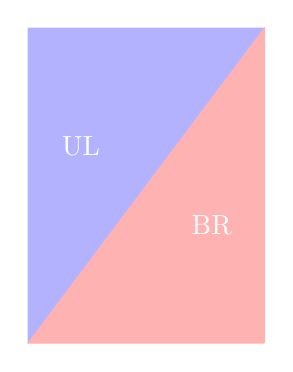
\begin{tikzpicture}
\draw[blue!30, fill= blue!30] (0,0) -- (3,4) -- (0,4) -- (0,0);
\draw[red!30,fill =red!30] (3,0) -- (3,4) -- (0,0) -- (3,0);
\node(A) at (0.67,2.5){\color{white} UL};
\node(B) at (2.33,1.5){\color{white} BR};
\end{tikzpicture}

{\it \footnotesize Figure 1: Box for determining consonant order.}
\end{center}

If the smaller line is in the upper-left triangle (UL), it the consonant it designates comes first. If it is in the bottom-right one, it comes second. For the rest of the explanation, it is advised to keep this box in the back of your head. An example:

\def\restorecorps{\renewcommand{\corpsgrootte}{20pt}}
\begin{wrapfigure}[7]{l}{0.4\textwidth}
\renewcommand{\corpsgrootte}{100pt}
\kus
\restorecorps
\end{wrapfigure}
\vspace{0.2cm}

As you see here, the smaller line is found on top. Hence, it is placed inside the upper-left triangle. The consonant for which the smaller horizontal line stands (the {\it k}), comes before the other consonant, the {\it s}.

\phantom{}

\begin{center}
\definecolor{melon}{RGB}{255,179,179}
\definecolor{caian}{RGB}{204,255,247}
\definecolor{lavender}{RGB}{242,179,255}
\definecolor{jasmine}{RGB}{255,212,128}
\definecolor{lemon}{RGB}{255,247,204}
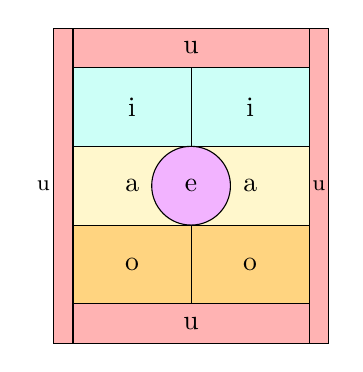
\begin{tikzpicture}
\draw[black] (0,0) rectangle (3,4);
\draw[fill = melon] (0,4) rectangle (3,3.5);
\draw[fill = melon] (0,0.5) rectangle (3,0);
\draw[fill = melon] (-0.25, 0) rectangle (0,4);
\draw[fill = melon] (3.25, 0) rectangle (3,4);
\draw[fill = caian] (1.5,2.5) rectangle (0,3.5);
\draw[fill = caian] (1.5,2.5) rectangle (3,3.5);
\draw[fill = jasmine] (1.5,1.5) rectangle (0,0.5);
\draw[fill = jasmine] (1.5,1.5) rectangle (3,0.5);
\draw[fill = lemon] (1.5,1.5) rectangle (0,2.5);
\draw[fill = lemon] (1.5,1.5) rectangle (3,2.5);
\draw[fill = lavender] (1.5,2) circle (0.5);
\node at (1.5,3.75){u};
\node at (0.75,3){i};
\node at (2.25,3){i};
\node at (0.75,2){a};
\node at (2.25,2){a};
\node at (0.75,1){o};
\node at (2.25,1){o};
\node at (1.5,0.25){u};
\node at (1.5,2){e};
\node at (-0.375, 2){\footnotesize u};
\node at (3.125, 2){\footnotesize u};
\end{tikzpicture}
\end{center}

{\footnotesize \it Figure 2: Location of the smaller line in relation to the vowel.}
\vspace{0.5cm}

The vowel is...
\begin{itemize}
\setlength{\itemsep}{0.25em}
\item {\it u\ }if the smaller line is found at the edges. The smaller line is in its whole above, under, left or right of the main line. 

\item {\it i\ } if the smaller line is found on the upper-left or upper-right side of the main line. It is usually smaller than the line made for {\it u}, to avoid confusion. 

\item {\it a\ } if the smaller line is found left or right to the middle of the line. 

\item {\it o\ } if the smaller line is found on the bottom-left or bottom-right hand of the main line. Again, this line is smaller than the line for {\it u}. 

\item{\it e\ } if the smaller line is placed in the middle. Or, if the small line intersects with the main line at the middle. In some instances, the small line is then split up by the main line.  
\end{itemize}

Then we have a single exception. You can combine two equivalent lines, to make syllables such as {\it pop}, {\it mum}, or {\it lol}. The order of these lines doesn't matter; hence we choose place the smaller line to the upper-left of the main line in such cases. For the vowel {\it u}, there are two small lines, split at the center. For {\it e}, there are either two or three small lines. At least one of those lines crosses through the center of the imaginary box.
%EXAMPLE>?

Remember that the {\it p} is represented by the dot $\bullet$\phantom{.}. For clarity, we couldn't combine simply two dots to make a full syllable. Hence, two p-dots combine a bit different from the rest of the lines. The p also can't combine well with the circle (which designated \lq\lq nothing \rq\rq). They combine in the following way:

\begin{center}
\renewcommand{\corpsgrootte}{10pt}
\begin{tabular}{c|c|c|c|c|c|c|}

\multicolumn{2}{l}{Basic line} & u & i & a & o & e\\ 
\hline
\phantom{M} & $\bullet$ & \up & \ip & \ap & \op & \ep \\

$\bullet$ & $\bullet$ & \pup & \pip & \pap & \pop & \pep \\

{$\bullet$} &  & \pu & \Atlanpi & \pa & \po & \pe\\
\end{tabular}
\end{center}
% \hspace{-0.30cm}\raisebox{-1.3em}{\renewcommand{\corpsgrootte}{40pt}\DeclareStroke{\Dot{Center}}\restorecorps}
\restorecorps

These were the rules for the script of Atlan. It might sound a bit cryptic, so let's discuss some examples. If you still feel uncertain whether you understand the rules, read through them again. Personal experience tells that, after some time, recognizing letters gets more intuitive. 

\pagebreak

\begin{wrapfigure}[7]{l}{0.4\textwidth}
\renewcommand{\corpsgrootte}{100pt}
\mok
\restorecorps
\end{wrapfigure}

\noindent Let's dissect this letter. This is the letter \lq\lq mok \rq\rq, or [PHONETICS] phonetically. First stept is to discover the main line, which is the long diagonal here. This is the consonant {\it m} ([phonetics]). Then there is a smaller line, found in the bottom-right corner. This is the {\it k} ([phonetics]). The horizontal line is in the bottom-right of our imaginary square. Hence, the {\it m} comes before the {\it k} (see also figure one). We got the two consonants, now rests the vowel. Feel free to look back at figure two. The smaller line is found in the bottom-right corner, hence the vowel here is an {\it o} ([phonetics]). The full syllable is {\it mok} ([Phonetics]). 


\begin{wrapfigure}[7]{r}{0.4\textwidth}
\renewcommand{\corpsgrootte}{100pt}
	\vspace{-1cm}
\jap
\restorecorps
\end{wrapfigure}

\vspace{0.2cm}
Now let's look at another one. See if you can determine the syllable yourself first. The main line is obvious: it's the big curve. This big curve is a {\it j\footnotemark} ([phonetics]). The smaller dot is a {\it p} ([Phonetics]). The dot is found inside the quadrant \lq\lq UL\rq\rq of figure one. Hence, the dot comes first. The dot is found a bit left from the centre of our imaginary box. Hence, the vowel here, is the {\it a} ([Phonetics]). The full syllable is jap ([phonetics]). 

\footnotetext{Quick tip: the curve for {\it j} looks alot like the {\it j} itself, doesn't it? Look for more of these similarities in our writing system; they help!}

\begin{wrapfigure}[7]{r}{0.4\textwidth}
\renewcommand{\corpsgrootte}{100pt}
\vspace{-0.5cm}
\lej
\restorecorps
\end{wrapfigure}


Do you feel if you got the hang of it? Let's do a few more. To spice things up a bit, we'll have a syllable with the vowel {\it e}. Remember that this vowel had smaller lines be placed in the centre. Alternatively, the smaller line could intersect the centre, or be split up by it. In this example, the smaller line is split up by the bigger line. The bigger line, the {\it l} ([PHonetics]) splits up the line for {\it j} ([Phonetics]). Because it does, the vowel is {\it e} ([phonetics]), and the syllable is {\it lej} ([phonetics]). 


\begin{wrapfigure}[7]{l}{0.4\textwidth}
\renewcommand{\corpsgrootte}{100pt}
\vspace{-0.5cm}
\pe
\restorecorps
\end{wrapfigure}

Now the last example. This, we think, is the best-looking glyph in our catalogue. What does it stand for? There aren't two, three, or four separate lines here, as should be. Instead, there is a triangle with a circle inside. What do we do? Well, remember the {\it p} ([Phonetics]), which was a dot. And remember that nothing also has it's line: the circle. There was an exeption for when two p-dots combined, or a p-dot and a circle. The exception was explained a few pages back. If you go there, you encounter the same glyph. This syllable is the {\it pe} ([phonetics]). A tip for remembering these glyphs: if you see a glyph with a triangle and a circle, think of the {\it p}.

We hope the examples have made clear how our writing system works. This concludes the explanation of our writing system for syllables. Upcoming is our writing system for numbers, and for names. Before we get to the next part, a few words of advice for learning the writing system:
\begin{itemize}
	\item On the next pages, a full list of our glyphs is added. They are 490 in number; as many glyphs as we have syllables. Don't be intimidated by the list; instead, use it wisely. Look through the list, and try to grasp the pattern of formation. Read the explanation above, and try to get a feel of how our glyps are formed. Again: after some while, you'll have a stronger intuition. 
	\item Try drawing some of the glyphs. It helps for getting used to the glyps. You don't need a ruler to draw them; just make sure they can be distinguished from each other. 
	\item Make some of the practice exercises in the back of the book! If you have worked through those, additional exercises can be found on our website, (WEBSITE). 
\end{itemize}

Again, on the next page is a table containing all our glyphs. The left two columns contain the base lines, placed in order of combination. If you've forgot which base line stands for which consonant, return to the table at the begin of the chapter. And, the $\empty$ means that the other line combines with nothing. 

\documentclass[landscape,a5paper]{article}
\usepackage{graphicx}
\usepackage{tikz}                                                                                                                                 
\usepackage{fancyhdr}
\usepackage[tmargin=20pt, bmargin=5pt, rmargin=20pt, margin=5pt]{geometry}
\usepackage{../Atlan}                                                                                                                                
\usepackage{fontspec}                                                                                                                             
\usepackage{longtable}                                                                                                                            
\usepackage[t,lf]{spectral}                                                                                                                       
\usepackage{geometry}                                                                                                                             
\pagestyle{empty}
\begin{document}
\newgeometry{tmargin=50pt, bmargin=5pt}
\fancyhead[R]{3.1. TYPOGRAPHY AND DIRECTION OF READING}
\fancyhead[L]{}

\let\newbullet\bullet
\renewcommand{\bullet}{\raisebox{0.3em}{\newbullet}}
\renewcommand{\corpsgrootte}{15pt}
\begin{longtable}{c c | c c c c c || c c | c c c c c}
	\multicolumn{2}{c}{Base lines} & u & i & a & o & e & \multicolumn{2}{c}{Base lines} & u & i & a & o & e \\
\hline

$\empty$ &  
$\empty$  &
\Atlanu &
\Atlani &
\Atlana &
\Atlano &
\Atlane & 
	&  & & & &  \\

$\empty$  &
\DeclareStroke{\CenterVertical} &
\ut &
\Atlanit &
\at &
\ot &
\et &

\DeclareStroke{\CenterVertical} &
$\empty$ & 
\tu &
\ti &
\ta &
\Atlanto &
\te \\

\DeclareStroke{\CenterVertical} &
\DeclareStroke{\CenterVertical} &
\tut &
\tit &
\tat &
\tot &
\tet &
  & & & & & \\

\DeclareStroke{\CenterVertical} &
\DeclareStroke{\CenterHorizontal} &
\tuk &
\tik &
\tak &
\tok &
\tek &

\DeclareStroke{\CenterHorizontal} &
\DeclareStroke{\CenterVertical} &
\kut &
\kit &
\kat &
\kot &
\ket \\
 
\DeclareStroke{\CenterVertical} &
\DeclareStroke{\RightDiagonal} &
\tun &
\tin &
\Atlantan &
\ton &
\ten &

\DeclareStroke{\RightDiagonal} &
\DeclareStroke{\CenterVertical} &
\nut &
\nit &
\nat &
\Atlannot &
\net  \\



\DeclareStroke{\CenterVertical} &
\DeclareStroke{\LeftDiagonal} &
\tum &
\tim &
\tam &
\tom &
\tem &

\DeclareStroke{\LeftDiagonal} &
\DeclareStroke{\CenterVertical} &
\mut &
\Atlanmit &
\mat &
\mot &
\met \\

\DeclareStroke{\CenterVertical} &
\DeclareStroke{\BigSE} &
\tuf &
\tif &
\taf &
\tof &
\tef &

\DeclareStroke{\BigSE} &
\DeclareStroke{\CenterVertical} &
\fut &
\fit &
\fat &
\fot &
\fet \\

\DeclareStroke{\CenterVertical} &
\DeclareStroke{\BigSW} &
\tus &
\tis &
\tas &
\tos &
\tes &

\DeclareStroke{\BigSW} &
\DeclareStroke{\CenterVertical} &
\sut &
\sit &
\sat &
\sot &
\set \\

\DeclareStroke{\CenterVertical} &
\DeclareStroke{\BigNE} &
\tul &
\til &
\tal &
\tol &
\tel &

\DeclareStroke{\BigNE} &
\DeclareStroke{\CenterVertical} &
\lut &
\lit &
\lat &
\lot &
\Atlanlet \\

\DeclareStroke{\CenterVertical} &
\DeclareStroke{\BigNW} &
\tuj &
\tij &
\taj &
\toj &
\tej &

\DeclareStroke{\BigNW} &
\DeclareStroke{\CenterVertical} &
\jut &
\jit &
\jat &
\Atlanjot &
\jet \\

\DeclareStroke{\CenterVertical} &
$\bullet$ &
\tup &
\tip &
\tap &
\Atlantop &
\tep &

$\bullet$ &
\DeclareStroke{\CenterVertical} &
\Atlanput &
\pit &
\pat &
\pot &
\pet \\


$\empty$ &
\DeclareStroke{\CenterHorizontal} &
\uk &
\ik &
\ak &
\ok &
\ek &

\DeclareStroke{\CenterHorizontal} &
$\empty$ &
\ku &
\ki &
\ka &
\ko &
\ke \\

\DeclareStroke{\CenterHorizontal} &
\DeclareStroke{\CenterHorizontal} &
\kuk &
\kik &
\kak &
\kok &
\kek &
 & & & & & \\


\DeclareStroke{\CenterHorizontal} &
\DeclareStroke{\RightDiagonal} &
\kun &
\kin &
\kan &
\kon &
\ken &

\DeclareStroke{\RightDiagonal} &
\DeclareStroke{\CenterHorizontal} &
\nuk &
\nik &
\nak &
\nok &
\nek \\


\DeclareStroke{\CenterHorizontal} &
\DeclareStroke{\LeftDiagonal} &
\kum &
\kim &
\kam &
\kom &
\kem &

\DeclareStroke{\LeftDiagonal} &
\DeclareStroke{\CenterHorizontal} &
\muk &
\mik &
\mak &
\mok &
\mek \\

\DeclareStroke{\CenterHorizontal} &
\DeclareStroke{\BigSE} &
\kuf &
\kif &
\kaf &
\kof &
\kef &

\DeclareStroke{\BigSE} &
\DeclareStroke{\CenterHorizontal} &
\fuk &
\fik &
\fak &
\fok &
\fek \\

\DeclareStroke{\CenterHorizontal} &
\DeclareStroke{\BigSW} &
\kus &
\kis &
\kas &
\kos &
\kes &

\DeclareStroke{\BigSW} &
\DeclareStroke{\CenterHorizontal} &
\suk &
\sik &
\sak &
\sok &
\sek \\

\DeclareStroke{\CenterHorizontal} &
\DeclareStroke{\BigNE} &
\kul &
\kil &
\kal &
\kol &
\kel &

\DeclareStroke{\BigNE} &
\DeclareStroke{\CenterHorizontal} &
\luk &
\lik &
\lak &
\lok &
\lek \\

\end{longtable}

\pagebreak

\newgeometry{tmargin=20pt, bmargin=30pt}

\begin{longtable}{c c | c c c c c || c c | c c c c c}
\multicolumn{2}{c}{Base lines} & u & i & a & o & e &  \multicolumn{2}{c}{Base lines} & u & i & a & o & e \\
\hline



\DeclareStroke{\CenterHorizontal} &
\DeclareStroke{\BigNW} &
\kuj &
\kij &
\kaj &
\koj &
\kej &

\DeclareStroke{\BigNW} &
\DeclareStroke{\CenterHorizontal} &
\juk &
\jik &
\jak &
\jok &
\jek \\

\DeclareStroke{\CenterHorizontal} &
$\bullet$ &
\kup &
\kip &
\kap &
\kop &
\kep &

$\bullet$ &
\DeclareStroke{\CenterHorizontal} &
\puk &
\pik &
\pak &
\pok &
\pek \\

$\empty$ &
\DeclareStroke{\RightDiagonal} &
\un &
\Atlanin &
\an &
\on &
\en &

\DeclareStroke{\RightDiagonal} &
$\empty$ &
\Atlannu &
\Atlanni &
\na &
\no &
\Atlanne \\

\DeclareStroke{\RightDiagonal} &
\DeclareStroke{\RightDiagonal} &
\nun &
\nin &
\nan &
\non &
\nen \\

\DeclareStroke{\RightDiagonal} &
\DeclareStroke{\LeftDiagonal} &
\num &
\nim &
\nam &
\nom &
\nem &

\DeclareStroke{\LeftDiagonal} &
\DeclareStroke{\RightDiagonal} &
\mun &
\Atlanmin &
\man &
\mon &
\men \\

\DeclareStroke{\RightDiagonal} &
\DeclareStroke{\BigSE} &
\nuf &
\nif &
\naf &
\nof &
\nef &

\DeclareStroke{\BigSE} &
\DeclareStroke{\RightDiagonal} &
\fun &
\fin &
\fan &
\fon &
\fen \\

\DeclareStroke{\RightDiagonal} &
\DeclareStroke{\BigSW} &
\nus &
\nis &
\nas &
\nos &
\nes &

\DeclareStroke{\RightDiagonal} &
\DeclareStroke{\BigSW} &
\sun &
\Atlansin &
\san &
\son &
\sen \\

\DeclareStroke{\RightDiagonal} &
\DeclareStroke{\BigNE} &
\nul &
\Atlannil &
\nal &
\nol &
\nel &

\DeclareStroke{\BigNE} &
\DeclareStroke{\RightDiagonal} &
\lun &
\lin &
\lan &
\lon &
\len \\

\DeclareStroke{\RightDiagonal} &
\DeclareStroke{\BigNW} &
\nuj &
\nij &
\naj &
\noj &
\nej &

\DeclareStroke{\BigNW} &
\DeclareStroke{\RightDiagonal} &
\jun &
\jin &
\jan &
\jon &
\jen \\

\DeclareStroke{\RightDiagonal} &
$\bullet$ &
\nup &
\nip &
\nap &
\nop &
\nep &

$\bullet$ &
\DeclareStroke{\RightDiagonal} &
\pun &
\pin &
\pan &
\pon &
\pen \\

$\empty$ &
\DeclareStroke{\LeftDiagonal} &
\um &
\im &
\am &
\om &
\Atlanem &

\DeclareStroke{\LeftDiagonal} &
$\empty$ &
\Atlanmu &
\mi &
\ma &
\mo &
\me \\

\DeclareStroke{\LeftDiagonal} &
\DeclareStroke{\LeftDiagonal} &
\mum &
\mim &
\mam &
\mom &
\mem &
 & & & & & & \\

\DeclareStroke{\LeftDiagonal} &
\DeclareStroke{\BigSE} &
\muf &
\mif &
\maf &
\mof &
\mef &

\DeclareStroke{\BigSE} &
\DeclareStroke{\LeftDiagonal} &
\fum &
\fim &
\Atlanfam &
\fom &
\fem \\

\DeclareStroke{\LeftDiagonal} &
\DeclareStroke{\BigSW} &
\mus &
\mis &
\mas &
\mos &
\mes &

\DeclareStroke{\BigSW} &
\DeclareStroke{\LeftDiagonal} &
\Atlansum &
\Atlansim &
\sam &
\som &
\sem \\

\DeclareStroke{\LeftDiagonal} &
\DeclareStroke{\BigNE} &
\mul &
\mil &
\mal &
\mol &
\mel &
\DeclareStroke{\BigNE} &
\DeclareStroke{\LeftDiagonal} &
\lum &
\Atlanlim &
\lam &
\lom &
\lem \\

\DeclareStroke{\LeftDiagonal} &
\DeclareStroke{\BigNW} &
\muj &
\mij &
\maj &
\moj &
\mej &

\DeclareStroke{\BigNW} &
\DeclareStroke{\LeftDiagonal} &
\jum &
\jim &
\jam &
\jom &
\jem \\

\DeclareStroke{\LeftDiagonal} &
$\bullet$ &
\mup &
\mip &
\map &
\mop &
\mep &

$\bullet$ &
\DeclareStroke{\LeftDiagonal} &
\pum &
\pim &
\pam &
\pom &
\pem \\

$\empty$ &
\DeclareStroke{\BigSE} &
\uf &
\Atlanif &
\af &
\of &
\ef &

\DeclareStroke{\BigSE} &
$\empty$ &
\fu &
\Atlanfi &
\fa &
\fo &
\fe \\

\DeclareStroke{\BigSE} &
\DeclareStroke{\BigSE} &
\fuf &
\fif &
\faf &
\fof &
\fef &
  & & & & & \\

\end{longtable}

\pagebreak 
\newgeometry{tmargin=50pt, bmargin=5pt}

\fancyhead[R]{3.1. TYPOGRAPHY AND DIRECTION OF READING}
\fancyhead[L]{}

\begin{longtable}{c c | c c c c c || c c | c c c c c}
\multicolumn{2}{c}{Base lines} & u & i & a & o & e & \multicolumn{2}{c}{Base lines} & u & i & a & o & e \\
\hline

\DeclareStroke{\BigSE} &
\DeclareStroke{\BigSW} &
\fus &
\fis &
\fas &
\fos &
\fes &

\DeclareStroke{\BigSW} &
\DeclareStroke{\BigSE} &
\suf &
\sif &
\saf &
\sof &
\sef \\

\DeclareStroke{\BigSE} &
\DeclareStroke{\BigNE} &
\ful &
\fil &
\fal &
\fol &
\fel &

\DeclareStroke{\BigNE} &
\DeclareStroke{\BigSE} &
\luf &
\lif &
\laf &
\lof &
\lef \\

\DeclareStroke{\BigSE} &
\DeclareStroke{\BigNW} &
\fuj &
\fij &
\faj &
\foj &
\fej &

\DeclareStroke{\BigNW} &
\DeclareStroke{\BigSE} &
\juf &
\jif &
\jaf &
\jof &
\jef \\

\DeclareStroke{\BigSE} &
$\bullet$ &
\fup &
\fip &
\fap &
\fop &
\fep &

$\bullet$ &
\DeclareStroke{\BigSE} &
\puf &
\pif &
\paf &
\pof &
\pef \\

$\empty$ &
\DeclareStroke{\BigSW} &
\us &
\is &
\as &
\os &
\es &

\DeclareStroke{\BigSW} &
$\empty$ &
\su &
\sa &
\si &
\so &
\se \\

\DeclareStroke{\BigSW} &
\DeclareStroke{\BigSW} &
\sus &
\sis &
\sas &
\sos &
\ses &
  & & & & & \\

\DeclareStroke{\BigSW} &
\DeclareStroke{\BigNE} &
\sul &
\sil &
\sal &
\sol &
\sel &

\DeclareStroke{\BigNE} &
\DeclareStroke{\BigSW} &
\lus &
\lis &
\las &
\los &
\les \\

\DeclareStroke{\BigSW} &
\DeclareStroke{\BigNW} &
\suj &
\sij &
\saj &
\soj &
\sej &

\DeclareStroke{\BigSW} &
\DeclareStroke{\BigNW} &
\jus &
\jis &
\jas &
\jos &
\jes \\

\DeclareStroke{\BigSW} &
$\bullet$ &
\Atlansup &
\sip &
\sap &
\sop &
\sep &

$\bullet$ &
\DeclareStroke{\BigSW} &
\pus &
\pis &
\pas &
\pos &
\pes \\

$\empty$ &
\DeclareStroke{\BigNE} &
\ul &
\il &
\al &
\ol &
\el &

\DeclareStroke{\BigNE} &
$\empty$ &
\lu &
\li &
\la &
\lo &
\Atlanle \\

\DeclareStroke{\BigNE} &
\DeclareStroke{\BigNE} &
\lul &
\lil &
\lal &
\lol &
\lel &
 & & & & & \\

\DeclareStroke{\BigNE} &
\DeclareStroke{\BigNW} &
\luj &
\lij &
\laj &
\loj &
\lej &

\DeclareStroke{\BigNW} &
\DeclareStroke{\BigNE} &
\jul &
\jil &
\jal &
\jol &
\jel \\

\DeclareStroke{\BigNE} &
$\bullet$ &
\lup &
\lip &
\lap &
\lop &
\lep &

$\bullet$ &
\DeclareStroke{\BigNE} &
\pul &
\pil &
\pal &
\pol &
\pel \\

$\empty$ &
\DeclareStroke{\BigNW} &
\uj &
\Atlanij &
\aj &
\oj &
\ej &

\DeclareStroke{\BigNW} &
$\empty$ &
\ju &
\ji &
\ja &
\jo &
\je \\

\DeclareStroke{\BigNW} &
\DeclareStroke{\BigNW} &
\juj &
\jij &
\jaj &
\joj &
\jej &
 & & & & & \\

\DeclareStroke{\BigNW} &
$\bullet$ & 
\jup &
\jip &
\jap &
\jop &
\jep &

$\bullet$ & 
\DeclareStroke{\BigNW} &
\puj &
\pij &
\paj &
\poj &
\pej \\

$\empty$ &
$\bullet$ &
\up &
\ip &
\ap &
\op &
\ep &

$\bullet$ &
$\empty$ &
\pu &
\Atlanpi &
\pa &
\po &
\pe \\

$\bullet$ &
$\bullet$ &
\pup &
\pip &
\pap &
\pop &
\pep &
 & & & & & \\

\end{longtable}

\end{document}




\Section{Numerals and Mathematics}{}


\Section{Font in \TeX}{Jarno Smets}


\Section{On Dyslexia}{Stijn Janssens and Jonathan Roose}

\Section{Cartouche}{}


